\documentclass[14pt]{beamer}

% beamer definieert 'definition' al, maar dan engels :(
% fix van:
% http://tex.stackexchange.com/questions/38392/how-to-rename-theorem-or-lemma-in-beamer-to-another-language
\usepackage[dutch]{babel}
\uselanguage{dutch}
\languagepath{dutch}
\deftranslation[to=dutch]{Definition}{Definitie}
\deftranslation[to=dutch]{Example}{Voorbeeld}

\definecolor{todocolor}{rgb}{1, 0.3, 0.2}
\newcommand{\td}[1]{\colorbox{todocolor}{*\footnote{TODO: #1}}}
\newcommand{\from}{\leftarrow}

\usepackage{array}

\usepackage{graphicx}
\usepackage{float}
\usepackage{amssymb}
\usepackage{color}
\usepackage{listings}

%\newcommand{\id}{\text{id}}
\newcommand{\N}{\mathbb{N}}
\newcommand{\Z}{\mathbb{Z}}
\newcommand{\R}{\mathbb{R}}
\newcommand{\cat}[1]{\mathbf{#1}}
\newcommand{\Ab}{\cat{Ab}}
\newcommand{\sAb}{\cat{sAb}}
\newcommand{\Set}{\cat{Set}}
\newcommand{\Ch}[1]{\mathbf{Ch}(#1)}
\newcommand{\Hom}[3]{\mathbf{Hom}_{#1}(#2, #3)}
\newcommand{\id}{\mathbf{id}}

\newcommand{\iso}{\cong}
\newcommand{\tot}[1]{\xrightarrow{\,\,{#1}\,\,}}
\newcommand{\eps}{\varepsilon}
\newcommand{\I}{\,\mid\,}
\newcommand{\then}{\Rightarrow}
\newcommand{\inject}{\hookrightarrow}
\newcommand{\del}{\partial}
\newcommand{\nsubgrp}{\trianglelefteq}

% relative to the one who includes us :(
\graphicspath{ {../images/} }

\newcommand{\todo}[1]{
	\addcontentsline{tdo}{todo}{\protect{#1}}
	$\ast$ \marginpar{\tiny $\ast$ #1}
}
\makeatletter
	\newcommand \listoftodos{\section*{Todo list} \@starttoc{tdo}}
	\newcommand\l@todo[2]{
		\par\noindent \textit{#2}, \parbox{10cm}{#1}\par
	}
\makeatother

\graphicspath{ {../presentation2/images/} {../thesis/images/} }

\title{Dold-Kan correspondentie
	\huge $$ \Ch{\Ab} \simeq \sAb $$}
\author{Joshua Moerman}
\institute[Radboud Universiteit Nijmegen]{Begeleid door Moritz Groth}
\date{}

\begin{document}


\begin{frame}
	\titlepage
\end{frame}

\begin{frame}
	Een \emph{categorie} $\cat{C}$ bestaat uit
	
	\vspace{5cm}\td{plaatje}

	met compositie $-\circ-$, zodat
	\begin{itemize}
		\item er is een identiteit $\id_c: C \to C$ en
		\item compositie is associatief.
	\end{itemize}
\end{frame}

\begin{frame}
	\frametitle{Voorbeelden}
	\begin{itemize}
		\item[$\Set$]
			objecten: verzamelingen \\
			pijlen: functies
		\item[$\Ab$]
			objecten: abelse groepen \\
			pijlen: groupshomomorfismes
		\item[$\underline{4}$] \td{diagram}
	\end{itemize}
\end{frame}

\begin{frame}
	\frametitle{Functors}
	Een \emph{functor} $F$ is een functie van een categorie $\cat{C}$ naar $\cat{D}$ op objecten \'en pijlen.

	\vspace{3cm}\td{plaatje}

	Zodat
	\begin{itemize}
		\item $F(\id_C) = \id_{F(C)}$ en
		\item $F(g \circ f) = F(g) \circ F(f)$.
	\end{itemize}
\end{frame}

\begin{frame}
	\frametitle{Voorbeeld functor}

	Voor een verzameling $V$ definieer
	$$ \Z[V] = \{ \phi: V \to \Z \I \phi(v) \neq 0 \text{ voor eindig veel } v \}. $$

	\bigskip
	Voor een functie $f: V \to W$ definieer
	\begin{gather*}
		\Z[f]: \Z[V] \to \Z[W] \\
		\Z[f](\phi) = \sum_v \phi(v) e_{f(v)}.
	\end{gather*}

	\bigskip
	Dit is een functor: $\Z[-]: \Set \to \Ab$.
\end{frame}

\begin{frame}
	\frametitle{Voorbeeld functor}

	\td{Commuterend diagram}
\end{frame}

\begin{frame}
	\frametitle{Samenvattend}
	\begin{itemize}
		\item Categorie $\stackrel{D}{=}$ objecten + pijlen.
		\item Functor $\stackrel{D}{=}$ pijl tussen categorie\"en.
	\end{itemize}

	\begin{itemize}
		\item Functor $\sim$ Constructies.
		\item Functor $\sim$ Diagrammen.
	\end{itemize}

	$F$ is \emph{contravariant} (notatie $F: \cat{C}^{op} \to \cat{D}$) als \\
	\td{plaatje}
\end{frame}

\begin{frame}
	\frametitle{D\'e categorie van mijn scriptie}

	\begin{itemize} \item[$\DELTA$]
			heeft als objecten $[n] = \{0, \ldots, n\}$, $n\in\N$ \\
			en als pijlen monotoon stijgende functies.
	\end{itemize}

	\only<1>{\begin{example}
		Voor elke $n$ zijn er pijlen
	\end{example}}
	\only<2->{\begin{lemma}
		Elke pijl in $\DELTA$ is een compositie van
	\end{lemma}}
	\begin{itemize}
		\item $\delta_i$\td{Definitie hier}
		\item $\sigma_i$
	\end{itemize}

	\visible<3>{
		Dus $\DELTA = \cdots$\td{Diagram hier}
	}
\end{frame}

\begin{frame}
	\frametitle{D\'e categorie van mijn scriptie}

	$\DELTA = \cdots$\td{Plaatje hier}

	\pause\bigskip
	\begin{lemma}
		Cosimpliciale gelijkheden\td{dingetjes}
	\end{lemma}
\end{frame}

\begin{frame}
\begin{center}
	\Large \visible<2->{$A:$} $\DELTA^{op} \to \Ab$ \visible<2->{\hspace{1cm}}

	\bigskip
	\visible<2->{
	$ A := $\td{diagram}
	}
\end{center}
\end{frame}

\begin{frame}
	\frametitle{De categorie $\sAb$}
	\begin{itemize}
		\item[Objecten] \emph{Simpliciaal abelse groepen} $A$ \\
		preciezer: functoren $A: \DELTA^{op} \to \Ab$
		\item[Pijlen] \emph{Natuurlijke transformaties} \\
		preciezer: $\phi: A \to B$ bestaat uit $\phi_n: A_n \to B_n$ zodat
		\vspace{2cm}\td{diagram}
	\end{itemize}
\end{frame}

\begin{frame}
	\frametitle{De categorie $\Ch{\Ab}$}
	\begin{itemize}
		\item[Objecten] \emph{Ketencomplexen} $C$ \\
		preciezer: collectie abelse groepen $C_n$ en groepshomonorfismes $\del_{n+1}: C_{n+1} \to C_n$ zodat $\del \circ \del = 0$
		\item[Pijlen] \emph{Ketenafbeeldingen} \\
		preciezer: $\phi: C \to D$ bestaat uit $\phi_n: C_n \to D_n$ zodat
		\vspace{2cm}\td{diagram}
	\end{itemize}
\end{frame}

\begin{frame}{$\sAb$ lijkt op $\Ch{\Ab}$}
Simpliciaal abelse groepen:
\begin{center}
	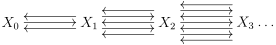
\includegraphics{simplicial_set} \\
	met de 5 vergelijkingen
\end{center}

Ketencomplexen:
\begin{center}
	$ C_0 \from C_1 \from C_2 \from \cdots $ \\
	met $\del \circ \del = 0$
\end{center}

\pause $\sAb$ heeft meer structuur?
\end{frame}

\begin{frame}{De Dold-Kan correspondentie}
	$$ \visible<2->{N:} \sAb \only<1>{\simeq} \only<2->{\rightleftarrows} \Ch{\Ab} \visible<2->{:K} $$
	
	\visible<2->{
	\begin{align*}
		\text{Zodat}\qquad &\forall C \in \Ch{\Ab}: &N(K(C)) \iso C \\
		\text{en}\qquad &\forall A \in \sAb: &K(N(A)) \iso A.
	\end{align*}
	}

	\bigskip\visible<3->{
	$N$ is in zekere zin surjectief: $\forall C \in \Ch{\Ab}$ is er een $A \in \sAb$ met $N(A) \iso C$.
	}
\end{frame}

\begin{frame}{Eerste gok}
	Definieer $M: \sAb \to \Ch{\Ab}$ met $M(A)_n = A_n$.

	\bigskip\pause
	Zij $C = \Z \from 0 \from 0 \from \cdots$\\
	Is er een $A$ zodat $M(A) \iso C$?\\
	M.a.w. $A_0 \iso \Z$ en $A_1 \iso 0$, kan dat?

	\bigskip\pause
	Nee! Want $A_0 \tot{A(\sigma_0)} A_1$ is injectief!\\
	(want $\sigma_0 \delta_0 = \id$, dus $A(\delta_0)A(\sigma_0) = \id$)
\end{frame}

\begin{frame}{Belangrijke definities}
	Zij $A \in \sAb$ \\
	$x \in A_n$ heet een \emph{$n$-simplex} \\
	$x$ is \emph{gedegenereerd} als $x = A(\sigma_i)(y)$ voor een zekere $i$ en $y$.

	\bigskip\pause
	\begin{lemma}
		$\forall x \in A_n$ \\
		$\exists !$ surjectie $\beta: [n] \epi [m]$ en\\
		niet-gedegenereerde $y \in A_m$ zodat
		$$ x = A(\beta)(y). $$
	\end{lemma}
\end{frame}

\begin{frame}{De juiste constructie}
	Zij $A \in \sAb$, definieer
	\begin{align*}
		N(A)_n &= \bigcap_{i=1}^n \ker(A(\delta_i)) \\
		\del &= A(\delta_0)
	\end{align*}

	\bigskip\pause
	\begin{lemma}
		$x \in N(A)_n$ is niet-gedegenereerd.
	\end{lemma}
	\bigskip
	\begin{lemma}
		Sterker nog:
		$$ A_n = N(A)_n \oplus D_n(A). $$
	\end{lemma}
\end{frame}

\begin{frame}
	\begin{center}
	\Huge Vragen?
	\end{center}
\end{frame}


\end{document}
